\clearpage
\subsubsection{\Optimizing MSVC + \olly}
\myindex{\olly}

We can try this (optimized) example in \olly.  Here is the first iteration:

\begin{figure}[H]
\centering
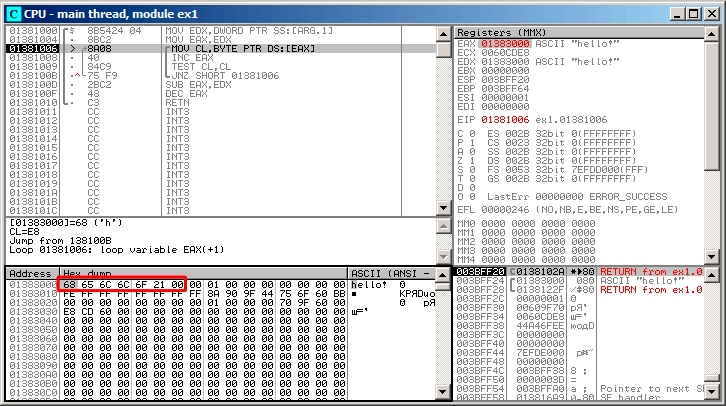
\includegraphics[scale=\FigScale]{patterns/10_strings/1_strlen/olly1.png}
\caption{\olly: first iteration start}
\label{fig:strlen_olly_1}
\end{figure}

We see that \olly found a loop and, for convenience, \IT{wrapped} its instructions in brackets.
By clicking the right button on \EAX, we can choose 
\q{Follow in Dump} and the memory window scrolls to the right place.
Here we can see the string \q{hello!} in memory.
There is at least
one zero byte after it and then random garbage.

If \olly sees a register with a valid address in it, that points to some string, 
it is shown as a string.

\clearpage
Let's press F8 (\stepover) a few times, to get to the start of the body of the loop:

\begin{figure}[H]
\centering
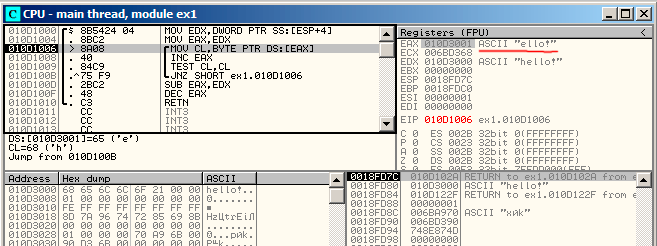
\includegraphics[scale=\FigScale]{patterns/10_strings/1_strlen/olly2.png}
\caption{\olly: second iteration start}
\label{fig:strlen_olly_2}
\end{figure}

We see that \EAX contains the address of the second character in the string.

\clearpage

We have to press F8 enough number of times in order to escape from the loop:

\begin{figure}[H]
\centering
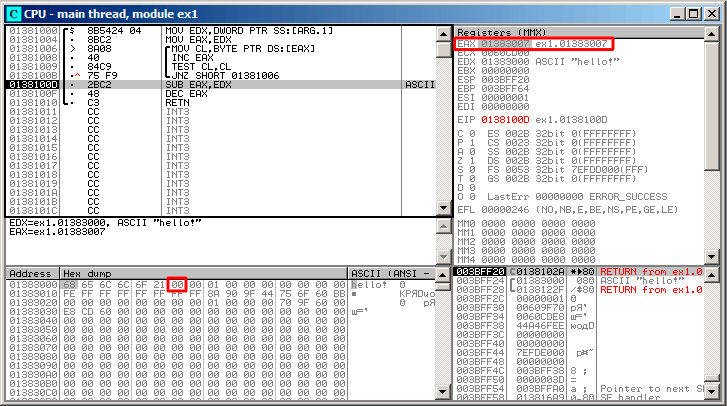
\includegraphics[scale=\FigScale]{patterns/10_strings/1_strlen/olly3.png}
\caption{\olly: pointers difference to be calculated now}
\label{fig:strlen_olly_3}
\end{figure}

We see that \EAX now contains the address of zero byte that's right after the string.
Meanwhile, \EDX hasn't changed,
so it still pointing to the start of the string.

The difference between these two addresses is being calculated now.

\clearpage
The \SUB instruction just got executed:

\begin{figure}[H]
\centering
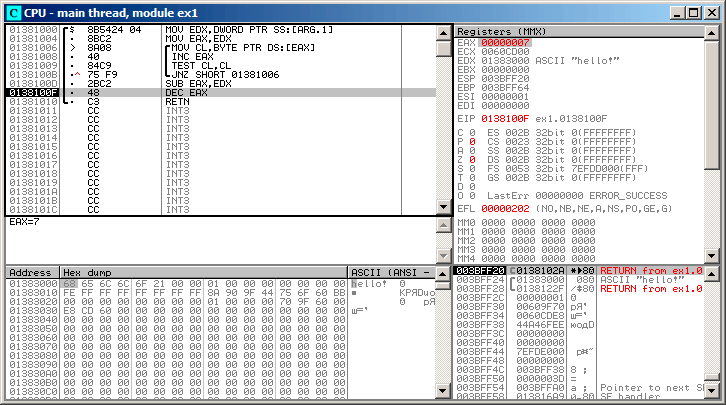
\includegraphics[scale=\FigScale]{patterns/10_strings/1_strlen/olly4.png}
\caption{\olly: \EAX to be decremented now}
\label{fig:strlen_olly_4}
\end{figure}

The difference of pointers is in the \EAX register now---7.
Indeed, the length of the \q{hello!} string is 6, 
but with the zero byte included\EMDASH{}7.
But \TT{strlen()} must return the number of non-zero characters in the string.
So the decrement executes and then the function returns.
